\section{World Of Warcraft}

\begin{figure}[htbp]
\begin{center}
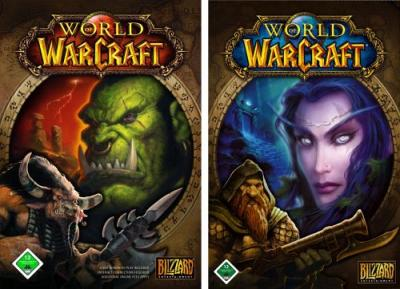
\includegraphics[width=.60\textwidth]{./imagenes/wowclasic.jpg}
\caption{World Of Warcraft}
\label{World Of Warcraft}
\end{center}
\end{figure}

World of Warcratf es uno de los mejores juegos online que existe a nivel mundial, la primera version de este juego fue lanzada en el año 2004 siendo denominada como Clásica, pocos años despues se fueron añadiendo nuevas expansiones, cada una de estas implementaron nuevos desafios y mejoras, haciendo que la gente quedara con la ganas de obtenerlo y jugarlo.

Una de las principales atracciones que obtuvo el juego fue la manera de implementar una gran cantidad de razas y clases, dentro de las que podemos definir las siguientes:

\large{Razas}
\begin{itemize}
\item Humano  \item Enano  \item Gnomo  \item Elfo de la noche 
\item Orco  \item No-muerto  \item Tauren  \item Trol
\end{itemize}

\large{Clases}
\begin{itemize}
\item Paladin  \item Chaman  \item Druida  \item Guerrero
\item Picaro  \item Sacerdote  \item Cazador  \item Brujo  \item Mago
\end{itemize}
\newpage
\begin{figure}[htbp]
\begin{center}
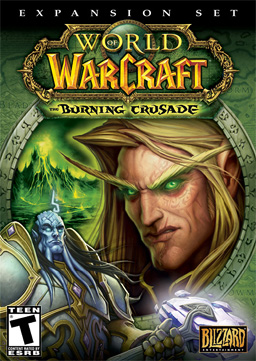
\includegraphics[width=.60\textwidth]{./imagenes/wowtbc.jpg}
\caption{World Of Warcraft: The Burning Crusade}
\label{World Of Warcraft: The Burning Crusade}
\end{center}
\end{figure}
La primera expansión lanzada en el año 2007, en el cual se implementaron 2 nuevas razas, una nueva ciudad,  un nuevo tipo de Campo de Batalla y un sistema de juego llamado Arenas. Ademas de que los Pjs podian alcanzan un nivel máximo de 70.

\begin{itemize}
\item Dranei
\item Elfo de sangre
\end{itemize}

\newpage
\begin{figure}[htbp]
\begin{center}
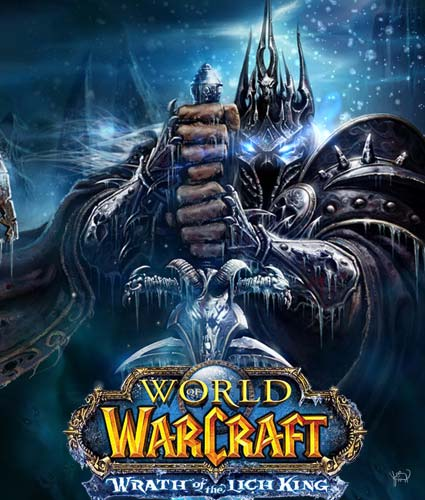
\includegraphics[width=.60\textwidth]{./imagenes/WOW.jpg}
\caption{World Of Warcraft: Wrath of the Lich King}
\label{World Of Warcraft: Wrath of the Lich King}
\end{center}
\end{figure}
Segunda expansión lanzada en el año 2008, dentro de esta la implementacion fue un nuevo continente Rasganorte, además de que se cuenta con llevar a los Pjs a un nivel de 80 y la implemtación de una nueva clase. Nuevas estancias de Mazmorras y Bandas fueron incluidas dentro de esta expansión por causa del nuevo continente.

\begin{itemize}
\item Caballero de la Muerte
\end{itemize}

\newpage
\begin{figure}[htbp]
\begin{center}
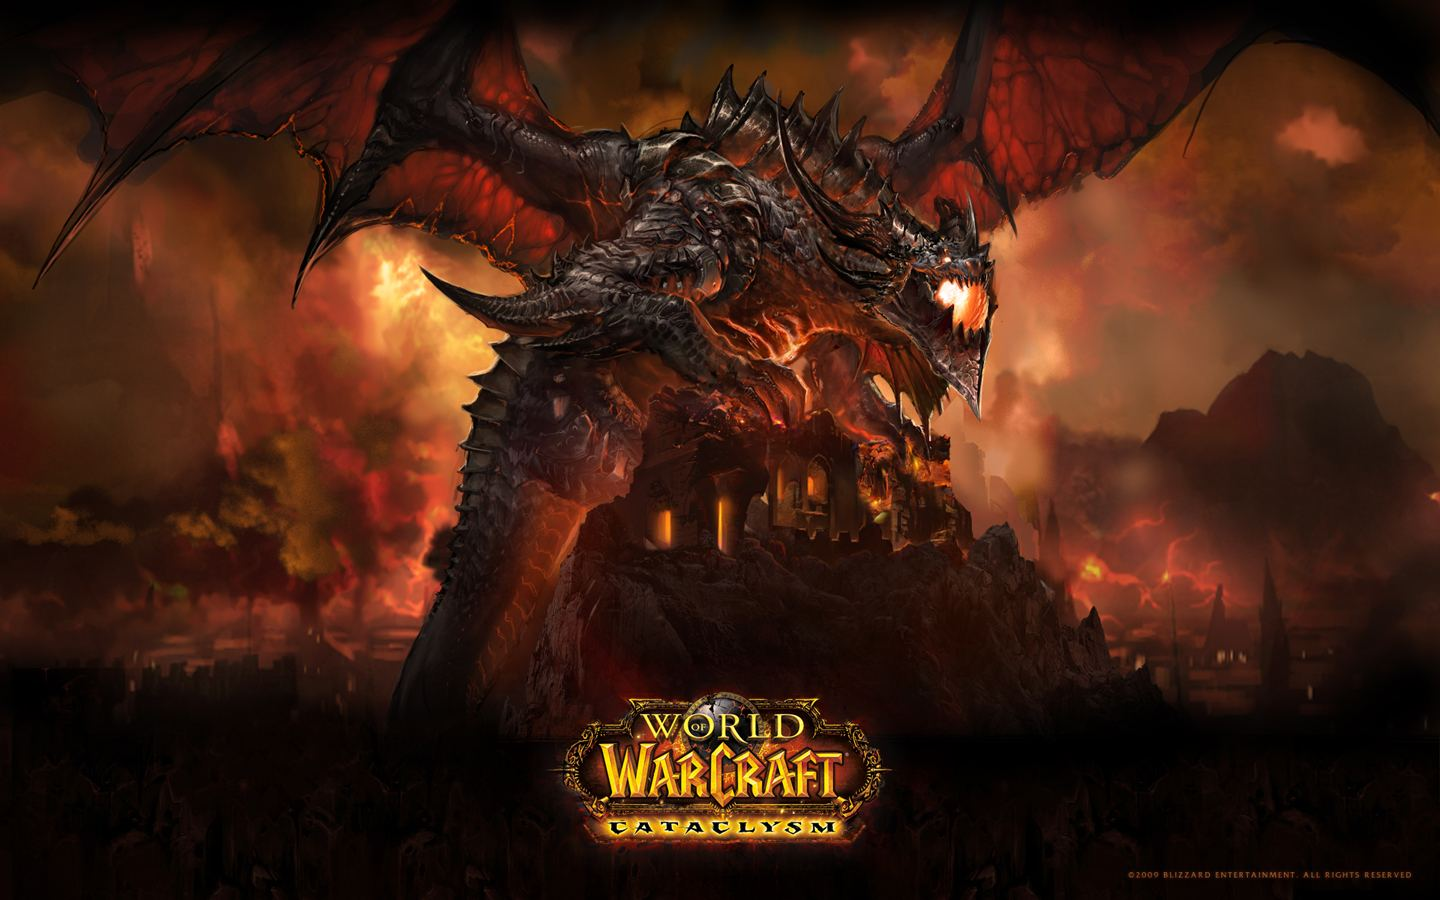
\includegraphics[width=.60\textwidth]{./imagenes/wowcataclysm.jpg}
\caption{World Of Warcraft: Cataclysm}
\label{World Of Warcraft: Cataclysm}
\end{center}
\end{figure}

Tercera expansión lanzada en el año 2010, la implementación para esta expansión fueron 1 nueva raza para cada facción, ademas de una nueva profesión secundaria y el nivel alcanza el 85. Las ciudades principales tanto de la Alianza como la Horda sufrieron cambios con respecto a sus aspectos.

\begin{itemize}
\item Huargen
\item Goblin

\item Arqueologia
\end{itemize}

\newpage
\begin{figure}[htbp]
\begin{center}
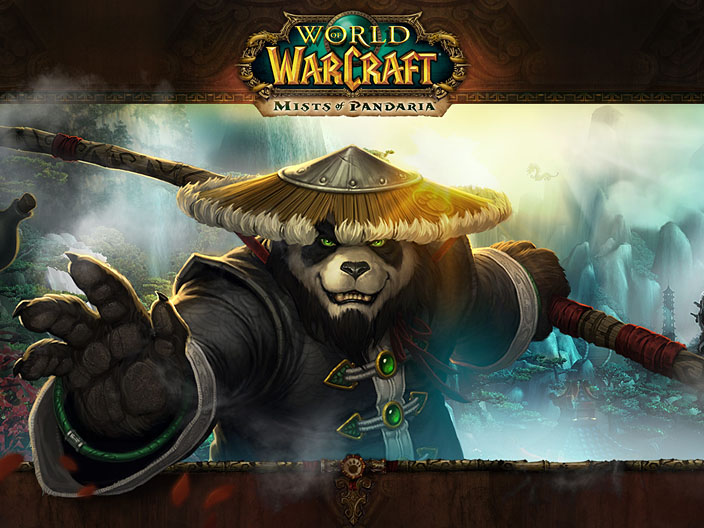
\includegraphics[width=.60\textwidth]{./imagenes/wowpandaren.jpg}
\caption{World Of Warcraft: Mists of Pandaria}
\label{World Of Warcraft: Mists of Pandaria}
\end{center}
\end{figure}
Cuarta y última expansión conocida actualmente, se inclyó una nueva raza junto con una nueva clase para las facciones, ademas de un nuevo continente, se cuenta con la implementación de nuevas mazmorras y desafios, en esta última expansión el limite de nivel es 90.

\begin{itemize}
\item Pandaren
\item Monje
\end{itemize}

Sufriendo muchos cambios durante cada expansión el juego tiende a convertirse en adictivo, a pesar de que ya no es el juego mas jugado en el mundo sigue estando con su record mundial.

\subsubsection{¿Por qué es uno de mis juegos favoritos?}
\begin{itemize}
\item[Marlon Loayza] La razón por la que es mi juego favorito se debe a la trama he historia que posee cada una de las razas dentro del juego, creando sus alianzas y combatiendo por el poder, la manera en la que te permite crear estrategias para la batalla es una de las razones mas fuertes de seguirlo jugando, ya que no luchas simplemente contra una maquina, cada jugador es una mente diferente y aplican diferentes tecnicas para combatir, haciendo que obtengas muchos desafios y te permite crear tus formas de jugar, la interacción virtual que haces con los demas jugadores hace que el juego sea mas entretenido ya que en ciertos casos estamos obligados a trabajar en grupos, lo que nos lleva a tener una buena comunicación. 
\end{itemize}
